\subsection{Molecular rotation}
\label{sec:mol-rotation}

Molecules have electronic and vibrational energy due to the motion of electrons and nuclei, respectively. Furthermore, they have rotational energy due to the overall rotation of the molecule. Like electronic and vibrational, rotational energy is quantized and generally has very small energies compared to the former.

\begin{figure}[!htb]
    \centering
    
    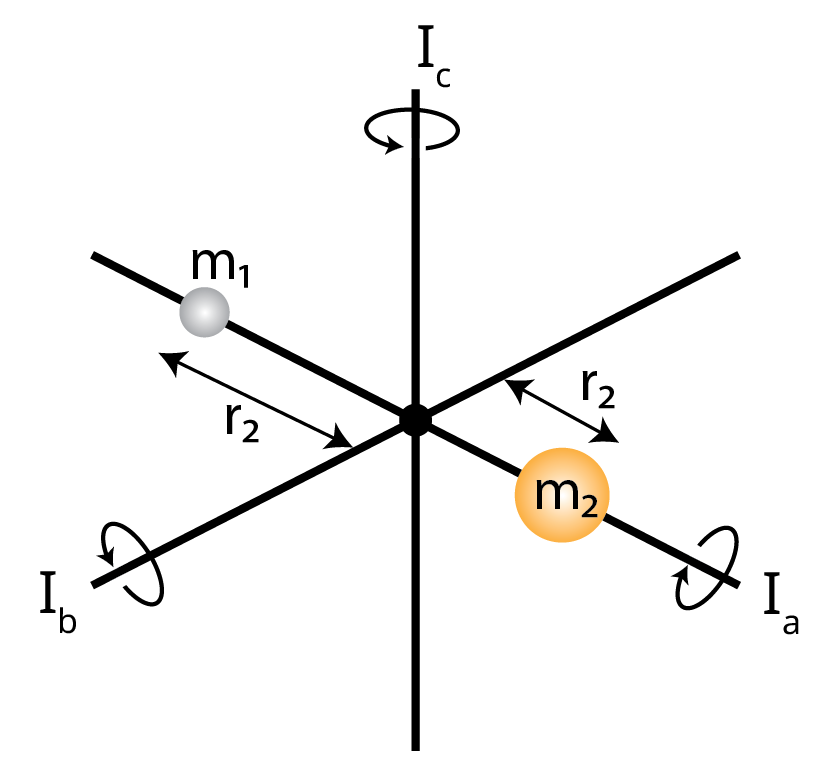
\includegraphics[scale=0.7]{figures/methods/rotation-rotor_linear.png}
    \caption{Rotation of linear molecule (heteronuclear diatomic) w.r.t principal rotational axis $a, b$ and $c$, with corresponding moment of inertia $I_a, I_b$ and $I_c$, respectively ($I_a$=0, $I_b$=$I_c$ for linear and diatomic molecules). $m$ and $r$ represent the mass of the atom and the distance to the rotating axis, respectively. The centre of mass lies at the origin.}
    \label{fig:rotor:diatomic}
\end{figure}

The molecules are classified according to their principal moments of inertia, $I_a, I_b$ and $I_c$, i.e., the moment of inertia along the principal rotational axis $a, b$ and $c$, respectively. The corresponding rotational constants are denoted as $A, B$ and $C$, respectively. The principal axes are perpendicular to each other and pass through the molecule's centre of mass (as shown in Figure \ref{fig:rotor:diatomic}). In general, the axes are conventionally defined such that: 

\begin{equation}
    \label{eqn:Iabc-reltion}
    I_a \leq I_b \leq I_c
\end{equation}

The moment of inertia, $I$, is defined as 

\begin{equation}
    \label{eqn:moment-of-inertia}
    I = \sum_i m_i r_i^2
\end{equation}

where $m_i$ and $r_i$ correspond to mass and distance to the rotating principal axis of atom $i$, respectively.

The main classifications are linear and non-linear molecules, while the latter is further divided, as will be briefly discussed in the following sections.

\subsubsection{Linear molecules}
\label{sec:mol-rotation:linear}

With a rigid rotor approximation, i.e., the bonds are rigid rods and molecule as a rigid rotor, the angular momentum is given by:

\[P_J = [J(J+1)]^{\frac{1}{2}} \hbar\]
where the rotational number $J=0, 1, 2, 3, ...$ .\\

In the presence of an electric or magnetic field,

\begin{equation}
    \label{eqn:rotation:MJ}
    (P_J)_z = M_J \hbar
\end{equation}

where, subscript $z$ represent z-axis component and $M_J = J, J-1, ..., -J$. This indicates that in the absence of an electric or magnetic field, each rotational level has $2J+1$ degenerate states.\\

The rotational energy ($E_r$) for a diatomic or linear polyatomic molecule can be solved using Eq. \ref{eqn:quantum:wave-eqn} and is given by:

\begin{equation}
    \label{eqn:rotational-energy-Er}
    E_r = \frac{h^2}{8\pi^2 I_b} J (J+1)
\end{equation}

The rotational energy in frequencies [Hz] can be defined using Eq. \ref{eqn:rotational-energy-Er}:

\begin{equation}
    \label{eqn:rotational-energy-FJ}
    F(J) = \frac{E_r}{h} = \frac{h}{8\pi^2 I_b} J(J+1) = BJ(J+1)
\end{equation}

where $F(J)$ is the rotational term values and $B$ is the rotational constant.\\
Only $B$ rotational constants are involved for linear molecules since as shown in Figure \ref{fig:rotor:diatomic}, $I_a=0$ and $I_b=I_c$.\\

The rigid rotor approximation does not hold true, especially in higher $J$ energy levels, because the chemical bonds expand due to centrifugal forces from molecular rotation. The expansion due to centrifugal force is included in equation \ref{eqn:rotational-energy-FJ} such that

\begin{equation}
    \label{eqn:rotational-energy-FJ-DJ}
    F(J) = BJ(J+1) -DJ^2(J+1)^2 + ...
\end{equation}

where $D$ is the centrifugal distortion constant. Eq. \ref{eqn:rotational-energy-FJ-DJ} also indicates that further higher-order terms may be included.

\subsubsection{Non-linear molecules}
\label{sec:mol-rotation:non-linear}
The non-linear molecules are further classified based on the principal moment of inertia. Analogous to $B$ rotational constant for linear molecule (Eq. \ref{eqn:rotational-energy-FJ}), the rotational constants $A, B$ and $C$ are given by:

\begin{equation}
    \label{eqn:rotational-constants}
    A=\frac{h}{8\pi^2 I_a};\ B=\frac{h}{8\pi^2 I_b};\ C=\frac{h}{8\pi^2 I_c}
\end{equation}

with units of frequency [Hz].\\

\textbf{Symmetric top: } It has two equal principal moments of inertia which corresponds to two possibilities: (a) $I_a < I_b = I_c$ and (b) $I_a = I_b < I_c$, these are called prolate and oblate, respectively. In symmetric tops, a second rotational quantum number $K=0, 1, 2, ..., J.$ is introduced in addition to $J$; therefore, Eq. \ref{eqn:rotational-energy-FJ} becomes

\begin{align}
    F(J, K) &= BJ(J+1) + (A-B)K^2\ \text{(prolate)} \label{eqn:rotational-energy-FJ-AKJ}\\
    F(J, K) &= BJ(J+1) + (C-B)K^2\ \text{(oblate)} \label{eqn:rotational-energy-FJ-CKJ}
\end{align}

The equations \ref{eqn:rotational-energy-FJ-AKJ} and \ref{eqn:rotational-energy-FJ-CKJ} indicate that for a particular value of $J$, the energy levels diverge and converge for a prolate and oblate symmetric tops, respectively. Since from Eq. \ref{eqn:Iabc-reltion} and \ref{eqn:rotational-constants}, we have $A \geq B \geq C$.\\

When the effect of centrifugal distortion is included, Eq. \ref{eqn:rotational-energy-FJ-DJ} becomes (for prolate),
\begin{equation}
    \label{eqn:rotational-energy-FJ-KJ}
    F(J, K) = BJ(J+1) + (A-B)K^2 - D_J J^2(J+1)^2 - D_{JK} J(J+1)K^2 - D_K K^4
\end{equation}

where there are now three centrifugal constants $D_J, D_{JK}$ and $D_K$.\\

\textbf{Spherical top: }It has all three principal moments of inertia equal, i.e., $I_a = I_b = I_c$. Therefore, the rotational term value follows the same as the equation for diatomic or linear polyatomic \ref{eqn:rotational-energy-FJ} and \ref{eqn:rotational-energy-FJ-DJ} (Section \ref{sec:mol-rotation:linear}).\\

\textbf{Asymmetric top: } It has all three principal moments of inertia unequal, i.e., $I_a \neq I_b \neq I_c $. Generally, the vast majority of molecules are asymmetric tops. But unfortunately, there are no analytical formulae for rotational term values for asymmetric tops molecules. $J$ is still a good quantum number, but $K$ is not, i.e., it does not take integral values. Therefore, only approximate expressions are derived, i.e., to approximate the molecule to either prolate or oblate near-symmetry top, such as:

\begin{align*}
    \begin{split}
        F(J, K) &\simeq B^* J(J+1) - (A-B^*)K^2\ \text{(near-prolate)} \\
        F(J, K) &\simeq B^* J(J+1) - (C-B^*)K^2\ \text{(near-oblate)}
    \end{split}
\end{align*}

where $B^*$ is equal to $\frac{1}{2} (B+C)$ for prolate and $\frac{1}{2} (A+C)$ for oblate rotor.

Since $K$ is not strictly a good quantum number and the $F(J, K)$ is only approximated.

\subsubsection{Selection rules}
\label{sec:mol-rotation:selection-rule}

Similar to the vibrational selection rule as discussed in Section \ref{sec:mol-vibration:selection-rule}, the rotational selection rule is determined from the rotational transition moment, $R_r$, defined as:

\[R_r = \int \psi_r^{'} \Vec{\mu} \psi^{''}\]

The rotational selection rule constitutes the condition for which $R_r$ is non-zero.\\

The selection rule:\\

for linear molecules and spherical top

\begin{enumerate}
\item $\Delta J = \pm 1$
\end{enumerate}

for symmetric top

\begin{enumerate}
\item $\Delta J = \pm 1$
\item $\Delta K = 0$
\end{enumerate}

for the asymmetric top

\begin{enumerate}
\item $\Delta J = 0, \pm 1$
\end{enumerate}

In addition to the above rules, all molecules must have a permanent electric dipole moment ($\Vec{\mu} \neq 0$) to observe rotational transition, and in the presence of the electric or magnetic field $\Delta M = 0, \pm 1$ (see Eq. \ref{eqn:rotation:MJ}).\\

The next section discusses relevant technical details for quantum chemical calculation employed in this thesis work.
